%----------------------- % - Academic Research - %-----------------------

\chapter{Academic Research}

\hypertarget{academicresearch}{}

%\begin{quote} \small "Human beings aren’t skeptical of arguments that give them
%exactly what they want, so bad arguments are often most interesting as indices
%of desire."

%\textemdash John Holbo,
%"\href{http://crookedtimber.org/2009/11/22/why-did-the-modernists-love-sans-serif/}{Why
%Did the Modernists Love Sans Serif?}"

%\end{quote}

\begin{quote} \small You are right to be wary. There is much bullshit. Be wary of me too, because
I may be wrong. Make up your own mind after you evaluate all the evidence and logic.

\textemdash Mark Rippetoe

\end{quote}

Research writing involves a number of important skills: library research,
critical thinking, the evaluation of sources, and the ability to synthesize
information through summary, paraphrase, and quotation. Although synthesizing
the thinking of others is an important part of the research essay, in its true
form the research essay strives for much more than a mere restatement of  what
others have said on a particular topic or question. As
\href{http://owl.english.purdue.edu/owl/resource/658/02/}{Jack Baker and Allen
Brizee} state:

\begin{quote}

A research paper is not simply an informed summary of a topic by
means of primary and secondary sources. It is neither a book report nor an
opinion piece nor an expository essay consisting solely of one's interpretation
of a text nor an overview of a particular topic. Instead, it is a genre that
requires one to spend time investigating and evaluating sources with the intent
to offer interpretations of the texts, and not unconscious regurgitations of
those sources. The goal of a research paper is not to inform the reader what
others have to say about a topic, but to draw on what others have to say about
a topic and engage the sources in order to thoughtfully offer a unique
perspective on the issue at hand.\end{quote}

\noindent In high school you were perhaps asked to write research papers on
predetermined  topics. These essays were probably not what Baker and Brizee have
in mind. Your  projects were likely just retellings of what other scholars or
writers have  said on a topic. A true research essay involves blazing a new path
of inquiry  where you produce original ideas, questions, and arguments. A
research paper is  a contribution to an ongoing conversation, a moment when you
engage in dialogue  with other important voices about a topic that you value.

\section{The Academic Conversation}

It is best to imagine a research essay as taking part in an ongoing
conversation. Unlike the dialogue that we have with most people in our lives,
these scholarly conversations occur in print\textemdash within published,
\hyperlink{peer-review}{\color{Ahrenge}{peer-reviewed}} books and journal articles. Some conversations are vibrant, with
hundreds or even thousands of participants. Other conversations are small,
involving but a few specialists. Many conversations have been going on for
hundreds or even thousands of years, while other conversations have only just started. Virtually everything you might write or think about is already part of
one or more of these conversations. So, even if you don't know it at the time,
when you write about anything you are entering a conversation that already
exists. 

Like any good conversationalist, the author of a research paper wants to
contribute his or her thoughts and opinions for the consideration of others in
the conversation. But if you want to be taken seriously in the conversation, you
have to know what the debates are about, who is involved in the dialogue, and
what has been said previously. In short, you must remain mindful that your ideas
have a \emph{context}. This is why research is important: it is how you come to understand what has already been said and by whom.

The moves you make in these conversations will take many forms. We might, for
example, take the idea of one scholar and build on it in some way\textemdash
perhaps by extending it to a new context. Or, we might offer a new
interpretation of the meaning of a particular film, historical event, or
scientific experiment. During this process of articulating our own views, we
often find ourselves in conflict with the thinking of others. As a result, we
will often contribute to the conversation by expressing why we disagree in part
or in whole with one or more of the other individuals in the conversation. In
any case, we must remain mindful that the conversation existed before we entered
it, and that whatever we might say or argue has a context that must be considered
and represented as we make our case. Thus, every academic paper you write will
not only argue an original point or idea, it will also show how that idea
emerges from a preexisting conversation.


\section{The Research Question}

Discovering your own research topic can be an overwhelming experience. With so
many things to choose from, finding a narrow focus is often difficult. However,
before you can truly begin your library research you need to find a way to
narrow your field of inquiry to a small set of research questions or problems.

At the outset your research questions will be rather general and mundane. But
that is perfectly normal: we all have to start somewhere. Once you have a
general topic of interest, however, you can move into a more rigorous research
phase.

As you begin your research, try to keep an open mind and allow yourself to be
pulled in new directions. It is important to think of the research process as
something more than a mere attempt to find information on a predetermined topic
or an effort to find evidence that supports an idea or belief that one already
holds, an error commonly referred to as \href{https://en.wikipedia.org/wiki/Confirmation_bias}{confirmation
bias}. Instead, research should be process of discovery where you encounter ideas and
contemplate questions that you would have otherwise never imagined. Research, done properly, has the power to change us\textemdash altering our views, values, and sense of things. But you must first allow yourself to become vulnerable to new ideas. During any particular research project you should be prepared to change your mind and your focus many, many times. You will frequently encounter dead ends; but you will also
experience the thrill of serendipitous discovery that will take you down a path
you would have never considered.

\section{Finding A Topic} \subsection{Exploring Topics with Subject Searches} If
you are having difficulty finding a narrow topic of interest, one way to get
started is to examine an organized list of \emph{every} subtopic that is
related to your broader subject. Since the
\href{http://catalog.loc.gov}{Library of Congress} assigns a series of
\textbf{subject headings} to every published book, you can easily browse a
meticulously categorized list of books that relate to your broader research
subject. For example, if you want to write an essay on the nation of Iraq, you
can perform a subject search with the search term "Iraq." The result will be an
alphabetized list of \emph{every} subject that scholars have written on about
Iraq\textemdash from agriculture to zoology. So, if you haven't yet found a
narrow focus for your project, you can use the subject headings to "shop" for a
subject that interests you.   \newpage

\subsection{Finding Additional Sources through Subject Searches} Subject
searches are also a helpful means of finding additional sources on your  topic
once you have acquired one or more. For example, if you discover that  historian
Alan Taylor's book \emph{\href{http://libcat.dartmouth.edu/record=b4878766}{The
Civil War of 1812}} is an important  source for your research project, you can
use the book's subject headings to  find \emph{all} of the other books written
on those topics. As you may see from this example on the right, the
Library of Congress  assigned the book the following three subject headings:

\begin{itemize}
\item{\small United States--History--War of 1812--Social aspects}

\item{\small Ontario--History--War of 1812--Social aspects}

\item{\small Northern boundary of the United States--History--19th century}
\end{itemize}

\noindent In most library catalogs these subject headings are hyperlinked;
clicking on  any of them leads you to a list of \emph{every} other book in the
library that shares  that particular subject heading. Thus, if your research
interest is the social aspects of the War of 1812, you can quickly find every
other book the library owns on that subject with a subject search.

Though Dartmouth's library holdings are not nearly as large as the Library of
Congress, you  can perform subject searches by selecting the \href{https://search.library.dartmouth.edu/discovery/search?vid=01DCL_INST:01DCL&mode=advanced}{advanced search} feature of the
\href{https://search.library.dartmouth.edu/}{library catalog}.

\subsection{Example of a Copyright Page}

\medskip

\begin{tcolorbox}[enhanced,width=4.2in,left=.4in, right=.4in,
   drop fuzzy shadow southeast,
    boxrule=0.4pt,sharp corners,colframe=black!80!black,colback=white!10]

\bigskip
\bigskip
\bigskip
\bigskip

\begin{center}

{\scriptsize FIRST VINTAGE BOOKS EDITION, OCTOBER 2011

\medskip

\emph{Copyright \copyright 2010 by Alan Taylor}

\medskip

All rights reserved. Published in the United States by Vintage Books,
a division of Random House, Inc., New York, and in Canada by
Random House of Canada Limited, Toronto. Originally published in hardcover in the Unted States by Alfred A. Knopf, a division of Random House, Inc., New York, in 2010.

\medskip

Vintage and colophon are registered trademarks of Random House, Inc.

\medskip

The Library of Congress has cataloged the Knopf edition as follows:

Taylor, Alan.

The civil war of 1812: American citizens, British subjects, Irish rebels, and Indian allies / Alan Taylor. \textemdash 1st. ed.

p. cm.

Includes bibliographical references and index.

1. United States\textemdash History\textemdash War of 1812\textemdash Social aspects.

2. Ontario\textemdash History\textemdash War of 1812\textemdash Social aspects.

3. Northern boundary of the United States\textemdash History\textemdash 19th century.

E354.T39 2010

973.5'2\textemdash dc22 2010012783

\textbf{Vintage ISBN: 978-0-679-77673-4}

\emph{Author photograph} \copyright \emph{Lynn Friedman}

\emph{Book design by Robert C Olsson}

www.vintagebooks.com

Printed in the United States of America

10 9 8 7 6 5 4 3 2 1

}


\end{center}
\bigskip
\smallskip
\smallskip

\end{tcolorbox}





\section{Finding Background Information}

A research project should always begin with the reading of general background
information about the topic. Before you can ask an intelligent question about
your topic or contribute to an ongoing scholarly conversation, you need to
develop a working knowledge of basic facts to serve as a foundation for your
project. The best way to develop this basic understanding is to examine
peer-reviewed reference works such as encyclopedias, dictionaries, and other
forms of \textbf{reference material}.

Baker-Berry library has a number of helpful reference resources in this regard.
If  you visit the  \href{http://researchguides.dartmouth.edu/reference}{Library Reference Resources} link in the Library's \href{http://researchguides.dartmouth.edu/}{Research Guides}, you
will find an impressive array of organized reference materials like
bibliographies, encyclopedias, and dictionaries. Most of them are fully
digitized and do not even require a trip to the library. Always start your
research project with reference works and gain a basic grounding of your topic
before developing your research question or thesis. For example, before you begin an essay on 
Iraqi feminism in the 1960s, you should read the wikipedia article on the modern history of Iraq to get
a broad sense of the context you are entering with your writing. Other helpful background information aids of note:

\begin{itemize}

\item \href{http://www.wikipedia.org}{Wikipedia}, \href{https://www.cia.gov/library/publications/the-world-factbook/}{CIA World Factbook}, \href{http://www.oxfordreference.com/}{Oxford Reference  Online}, \href{http://www.search.eb.com/}{Britannica Online}.

\end{itemize}

A word of warning about Wikipedia (and internet sources in
general): it has not  been through a process of \hyperlink{peer-review}{\color{Ahrenge}{peer review}}. For that
reason, it is unwise to rely on Wikipedia as a source for a research project. Use
Wikipedia to gain background information on your topic and lead you to other authoritative sources, but when it comes time to write your essay, use a peer-reviewed source.

\section{Research Guides}

Perhaps the single best aid for research at Dartmouth is the
\href{http://researchguides.dartmouth.edu}{Research Guide}. Various subject
librarians maintain research guides for every discipline. These guides contain
links to subject-specific reference materials (such as encyclopedias and
dictionaries),  appropriate peer-reviewed journals, electronic databases,
biographies, e-texts, book reviews, and a variety of other helpful resources and
tips. These guides should be your first stop on a research project and will be
an indispensable resource for discovering sources on your chosen topic. These guides are rather uneven. Some are quite excellent; others are rather skimpy. 

\section{Searching for Books}

When you want to search for books that Dartmouth library owns or can access
electronically, use the \href{http://libcat.dartmouth.edu/}{Library Catalog}.
Dartmouth also offers a more robust search tool known as
\href{https://search.library.dartmouth.edu/}{Primo}. Primo provides
you with an experience similar to Google; search terms are applied not only to
physical holdings, like books and media, but to electronic databases and journals as well.

Primo is used as the backend for the search field on the library's front page. After you submit your
search term in the field, you will be presented with a list of books, articles, databases, audio \& video, associated digital content, or research aids. These items are organized by relevance, as determined by an algorithm. After entering your search you will notice ways to further refine your search by clicking on several options on the left pane of the window. You might, for example, select for peer-reviewed content, limit your search to books/articles, or ensure that you only see content accessible through our library.  

\begin{center}
\begin{tcolorbox}[colframe=oyster, coltitle=black, sharp corners, title=\ding{52} Note]
\textbf{One word of caution about}
\href{https://search.library.dartmouth.edu/}{Primo}: while
it searches the library catalog it its entirety, it \emph{does not search all of
the electronic databases to which Dartmouth has a subscription}. This means that
if you exclusively use Primo for your searches, you will miss out on potentially vast amounts of possible sources that could be discovered through searching the various databases individually.
\end{tcolorbox}
\end{center}


\section{Searching for Periodicals/Articles}

Periodicals are publications that are published at regular intervals, such as
scholarly journals, magazines, and newspapers. Examining periodicals\textemdash
especially academic journals\textemdash is an important aspect of research.
Since books often take a year or more to go through the process of peer review,
editing, typesetting, and printing before they become available for purchase,
they often do not contain the most current information. Articles, on the other
hand, appear in a far shorter period of time and generally contain the most
up-to-date research. For that reason, you should perform a review of journal
articles on your research topic to ensure that you are aware of recent
discoveries, arguments, and debates within the academic community who share
your research focus.

However, a common problem for undergraduate researchers is not knowing which
databases or journals to search for information on a particular topic. Unless
you are a professional scholar, it is difficult to know what the leading
journals are in a particular field of study. This is also a problem for faculty performing research outside of their area of expertise. For example, an English professor would know that the academic journal \emph{PMLA} or the database JSTOR are excellent places to look for articles on Herman Melville's novel \emph{Moby
Dick}, but the novice researcher wouldn't know where to begin.

To resolve this problem, our library has organized periodical databases by
discipline in the \href{https://researchguides.dartmouth.edu/az.php}{Database
Finder}. This is designed to help you locate the specific journals, periodical
databases, and that are appropriate for each discipline or  research subject.
These are an indispensable resource for discovering  peer-reviewed sources on
your chosen topic.

You may also browse alphabetically if you know the name of the database you are
looking for.

\section{Searching with Precision}

A common research problem is that your searches produce too many results.
Rather than page through hundreds or thousands of search results, you should
become familiar with powerful \textbf{Boolean searches} to make your search
terms more precise. Boolean searches use what are known as \textbf{logical
operators} to form search terms. The three most common logical operators are
\textbf{AND}, \textbf{OR}, and \textbf{NOT}.

\subsection{AND}

Although it may seem counterintuitive, \textbf{AND} is used to \emph{narrow}
the number of sources you retrieve from a database. You can visualize  the
search of a large academic database or library catalog using the following
diagram:
\begin{center}
\begin{tikzpicture}
  \tikzset{venn circle/.style={draw,circle,minimum width=6cm,fill=#1,opacity=0.4,text opacity=1}}

  \node [venn circle = green] (A) at (0,0) {$cognitive$};
  \node [venn circle = white] (B) at (60:4cm) {$linguistics$};
  \node [venn circle = gray] (C) at (0:4cm) {$childhood$};
  \node[left] at (barycentric cs:A=1/2,B=1/2 ) {};
  \node[below] at (barycentric cs:A=1/2,C=1/2 ) {};
  \node[right] at (barycentric cs:B=1/2,C=1/2 ) {};
  \node at (barycentric cs:A=1/3,B=1/3,C=1/3 ) (endpoint) {};

  \draw[*-angle 60]
    ( [yshift=-20pt] $ (A.south)!0.5!(C.south) $ ) node[anchor=north] {\{ linguistics \textbf{AND} cognitive \textbf{AND} childhood \}}
    to[bend right,looseness=1]
    (endpoint.south east);
\end{tikzpicture}
%\begin{center} \includegraphics[width=.30\textwidth]{and3colors.png}
%\{ childhood \emph{AND} linguistics \emph{AND} cognitive \} \end{center}

\end{center}

\noindent In the search depicted above, a student has requested articles that
contain the  subjects \textbf{cognitive}, \textbf{linguistics}, and
\textbf{childhood}.  This particular search will only retrieve articles that
contain  \emph{all three terms}. This small subset of the larger subject sets is
referenced by the arrow. All the information represented by the other portions
of the three circles will be excluded. Thus, even if an article contains two of
the three search terms, it will be excluded from the results.

\subsection{OR} Unlike the \textbf{AND} operator, \textbf{OR} seeks to
\emph{broaden} a search,  as in this example:
\bigskip

\begin{center}
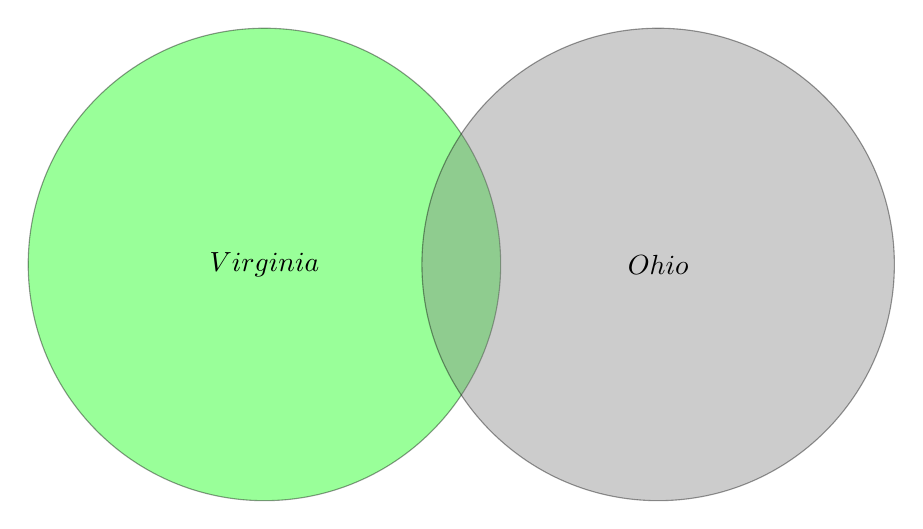
\begin{tikzpicture}
  [venn circle/.style={draw,circle,minimum width=6cm,fill=#1,opacity=0.4,text opacity=1}]

  \node [venn circle = green] (A) at (0,0) {$Virginia$};
  %\node [venn circle = white] (B) at (60:4cm) {$Ohio$};
  \node [venn circle = gray] (C) at (0:5cm) {$Ohio$};
  %\node[left] at (barycentric cs:A=1/2,B=1/2 ) {};

  \node[below] at (barycentric cs:A=1/3 ) (endpoint A) {};
  \node[below] at (barycentric cs:C=1/3 ) (endpoint C) {};

\end{tikzpicture}

\{ Virginia \textbf{OR} Ohio \}
\end{center}

%\begin{center} \includegraphics[width=.30\textwidth]{Orcolor.png}
%\{ Virginia \emph{or} Ohio \} \end{center}

\noindent In the search depicted above, a student has searched for the subjects
Virginia \textbf{OR} Ohio. This search will return \emph{every} article having
the  subject of Virginia as well as \emph{every} article with the subject of
Ohio.  Unlike the \textbf{AND} search, where only articles containing
\emph{both} terms are returned in the search results, the \textbf{OR} search
yields every source on both subjects regardless of whether those subjects
appear together in the same source. As a consequence, the \textbf{OR} search
will produce far more results.

\begin{itemize}\item Since the \textbf{OR} operator lacks precision, it is most
often used in parenthetical searches, described below.\end{itemize}

\subsection{NOT} The Boolean operator \textbf{NOT} is used to \emph{subtract} or
\emph{screen out} topics or keywords that are unwanted within the search
results.

\begin{center}

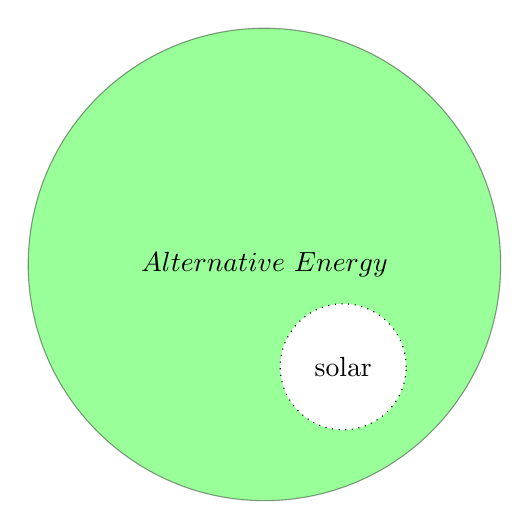
\begin{tikzpicture}
  \tikzset{venn circle/.style={draw,circle,minimum width=6cm,fill=#1,opacity=0.4,text opacity=1}}
  \node [venn circle = green] (A) at (0,0) {$Alternative \ Energy$};
  \path [draw=none,fill=white] (1,-1.3) circle (.8);
    \draw[dotted] (1,-1.3) circle (.8) node{solar};
    %\draw[solid] (0,-1) circle (2);
  %\node [venn circle = white] (B) at (60:4cm) {$Ohio$};
 % \node [venn circle = gray] (C) at (0:5cm) {$Ohio$};
  %\node[left] at (barycentric cs:A=1/2,B=1/2 ) {};
  %\node[below] at (barycentric cs:A=1/2,C=1/2 ) {};
  %\node[right] at (barycentric cs:B=1/2,C=1/2 ) {};
  %\node[below] at (barycentric cs:A=1/3 ) (endpoint) {};
 %  \node[below] at (barycentric cs:C=1/3 ) (endpoint) {};
  %\draw[*-angle 60]
   % ( [yshift=-10pt] $ (A.south)!0.5!(C.south) $ ) node[anchor=north] {\{ Virginia \emph{or} Ohio \}}
   % to[bend right,looseness=1.5]
   % (endpoint.south east);


\end{tikzpicture}


\{ alternative energy \textbf{NOT} solar \}

\end{center}

\noindent In the search depicted above, a student is researching alternative
energy and wants to exclude any information dealing with solar energy. To
remove all references to solar energy, the student has searched for
\textbf{alternative energy}, but has removed any articles from the search
results that contain the  subject \textbf{solar} using the operator
\textbf{NOT}.

The \textbf{NOT} operator is helpful when you find your search results are
"polluted" with unwanted items. This is often a problem when two distinct
things share the same name. For example, if you were researching the Norse
explorers known as the Vikings, you might discover that your search results
include unwanted information about the Minnesota Vikings football team. You can
subtract these unwanted results by searching for \textbf{Vikings NOT Minnesota}
or \textbf{Vikings NOT football}, for example.

\subsection{Parenthetical Searches}

You can also use the various Boolean search terms in tandem using parenthetical
constructions:

\begin{itemize} \item (Ohio OR Virginia) AND unemployment \item (cognitive AND
linguistics) NOT childhood \end{itemize} Such parenthetical searches follow the
order of operations, like in math  equations. In the first example, the search
will first combine all the articles  that are on the subjects of \textbf{Ohio}
or \textbf{Virginia}, creating a  large collection of search results. Afterward,
the search term  \textbf{unemployment} will be applied to that collection,
yielding the final search results. Similarly, the second example creates a
large collection of results that share the subjects \textbf{cognitive} and
\textbf{linguistics}, then all the items having the term \textbf{childhood}
are removed from the results.

\subsection{Exact Phrase Searches}

Most Internet search engines and library catalogs default to the \textbf{AND}
operator when multiple terms are entered, even if it has not been typed by the
user. For example, if you search for \textbf{artificial intelligence}, the
search algorithm will actually use the search phrase \textbf{artificial
\emph{and} intelligence} to produce your results. In some circumstances this
may produce undesirable or imprecise results. For example, we might imagine a scholarly article about the "intelligence" of using certain "artificial" sweeteners. This is not an article that is relevant for your research. 

To avoid this problem, you can instruct your search engine to perform what is
known as an \textbf{exact phrase search}. This is performed by placing
quotation marks around the exact words you are searching for. By searching
for "artificial intelligence" your search results will only contain items that
have that exact phrase within the document or title.

\subsection{Truncation and Wild Cards} \begin{itemize} \item manufact\**
[truncation] \item wom\**n [wild card] \end{itemize} If you search for the terms
\textbf{steel AND manufacturing}, your search  results may not include results
with the terms \textbf{manufacturer},  \textbf{manufacture},
\textbf{manufactured}, or \textbf{manufactures}. As a result, you may not
discover articles or books that are important to your research. By truncating
the word with an asterisk, you will gather all the relevant search results.

Similarly, if you only search for wom\hl{en}, you will potentially miss out on the
all the texts that mention wom\hl{an}. However, using the wild card
asterisk you will search both terms simultaneously, gathering all the results.

\section{Finding a Book in the Library}

\subsection{The Library of Congress System} Most research libraries use the
Library of Congress (LC) classification system to organize their holdings. The
Library of Congress assigns each book a unique \textbf{call number} consisting
of a series of numbers and letters that help  you locate them on the library's
shelves. A typical call number will resemble  the following:

\begin{center}
\bigskip

{\huge F 24 .T39 1990}
\end{center}

\bigskip

On a book's binding it will be written like this:

\begin{center}
{\huge F} \smallskip

{\huge 24}\smallskip

{\huge .T39}\smallskip

{\huge 1990}

\end{center}

\noindent Let's break down the call number into its component parts:

\bigskip

{\large
\begin{center}
\begin{tabular}{ ll }    \textbf{F} & Letter, or
subject, line \\    \textbf{24} & Whole number line \\     \textbf{.T39} & Cutter
line \\   \textbf{1990} & Edition, or Date, line\\  \end{tabular}
\end{center}
}
\medskip

\begin{itemize}

\item \textbf{The Letter line} describes the subject matter, or
discipline, of the book. It also indicates the section of the library where the
book is shelved (consult the library's \href{http://www.dartmouth.edu/~library/bakerberry/circ/stacksguides/}{floorplan
maps}). The letter line will be between one and three letters long. \item \textbf{The Whole number
line} tells you which \emph{row} the book is on in the stacks.  \item
\textbf{The Cutter line} identifies the \emph{individual book}. The first
letter of the Cutter line is usually the first letter of the author's last name.
\item \textbf{The Edition, or Date, line} tells you the book's year of
publication. This line is used to distinguish between editions.\bigskip

You can examine the \href{https://www.loc.gov/catdir/cpso/lcco/}{full list of subject classes} used by LC system online at the Library of Congress.\end{itemize}

\subsection{How to Find a Book} \smallskip

To find a book in the library, read the call number from left to right, using  alphabetical and
numerical orders. First, using the \textbf{Letter line},  determine the floor of
the library where the book is shelved. Use the library's
\href{http://www.dartmouth.edu/~library/bakerberry/circ/stacksguides/}{floorplan
maps}  to locate the proper section. Using our example call number above, we can
determine that the \textbf{F} section is in Stack Annex A.

Once on the appropriate floor, use the \textbf{Whole number line} to find the
row where the book is shelved in the stacks. Using the example call number, we
will look through the stacks for the number 24. The floormaps are often helpful
in locating the book's general location on the library floor. As you walk
through the stacks, look on the ends of each row of books for signs describing
the range of books held within the rows. There you will see signs like the one
pictured below.

\begin{center}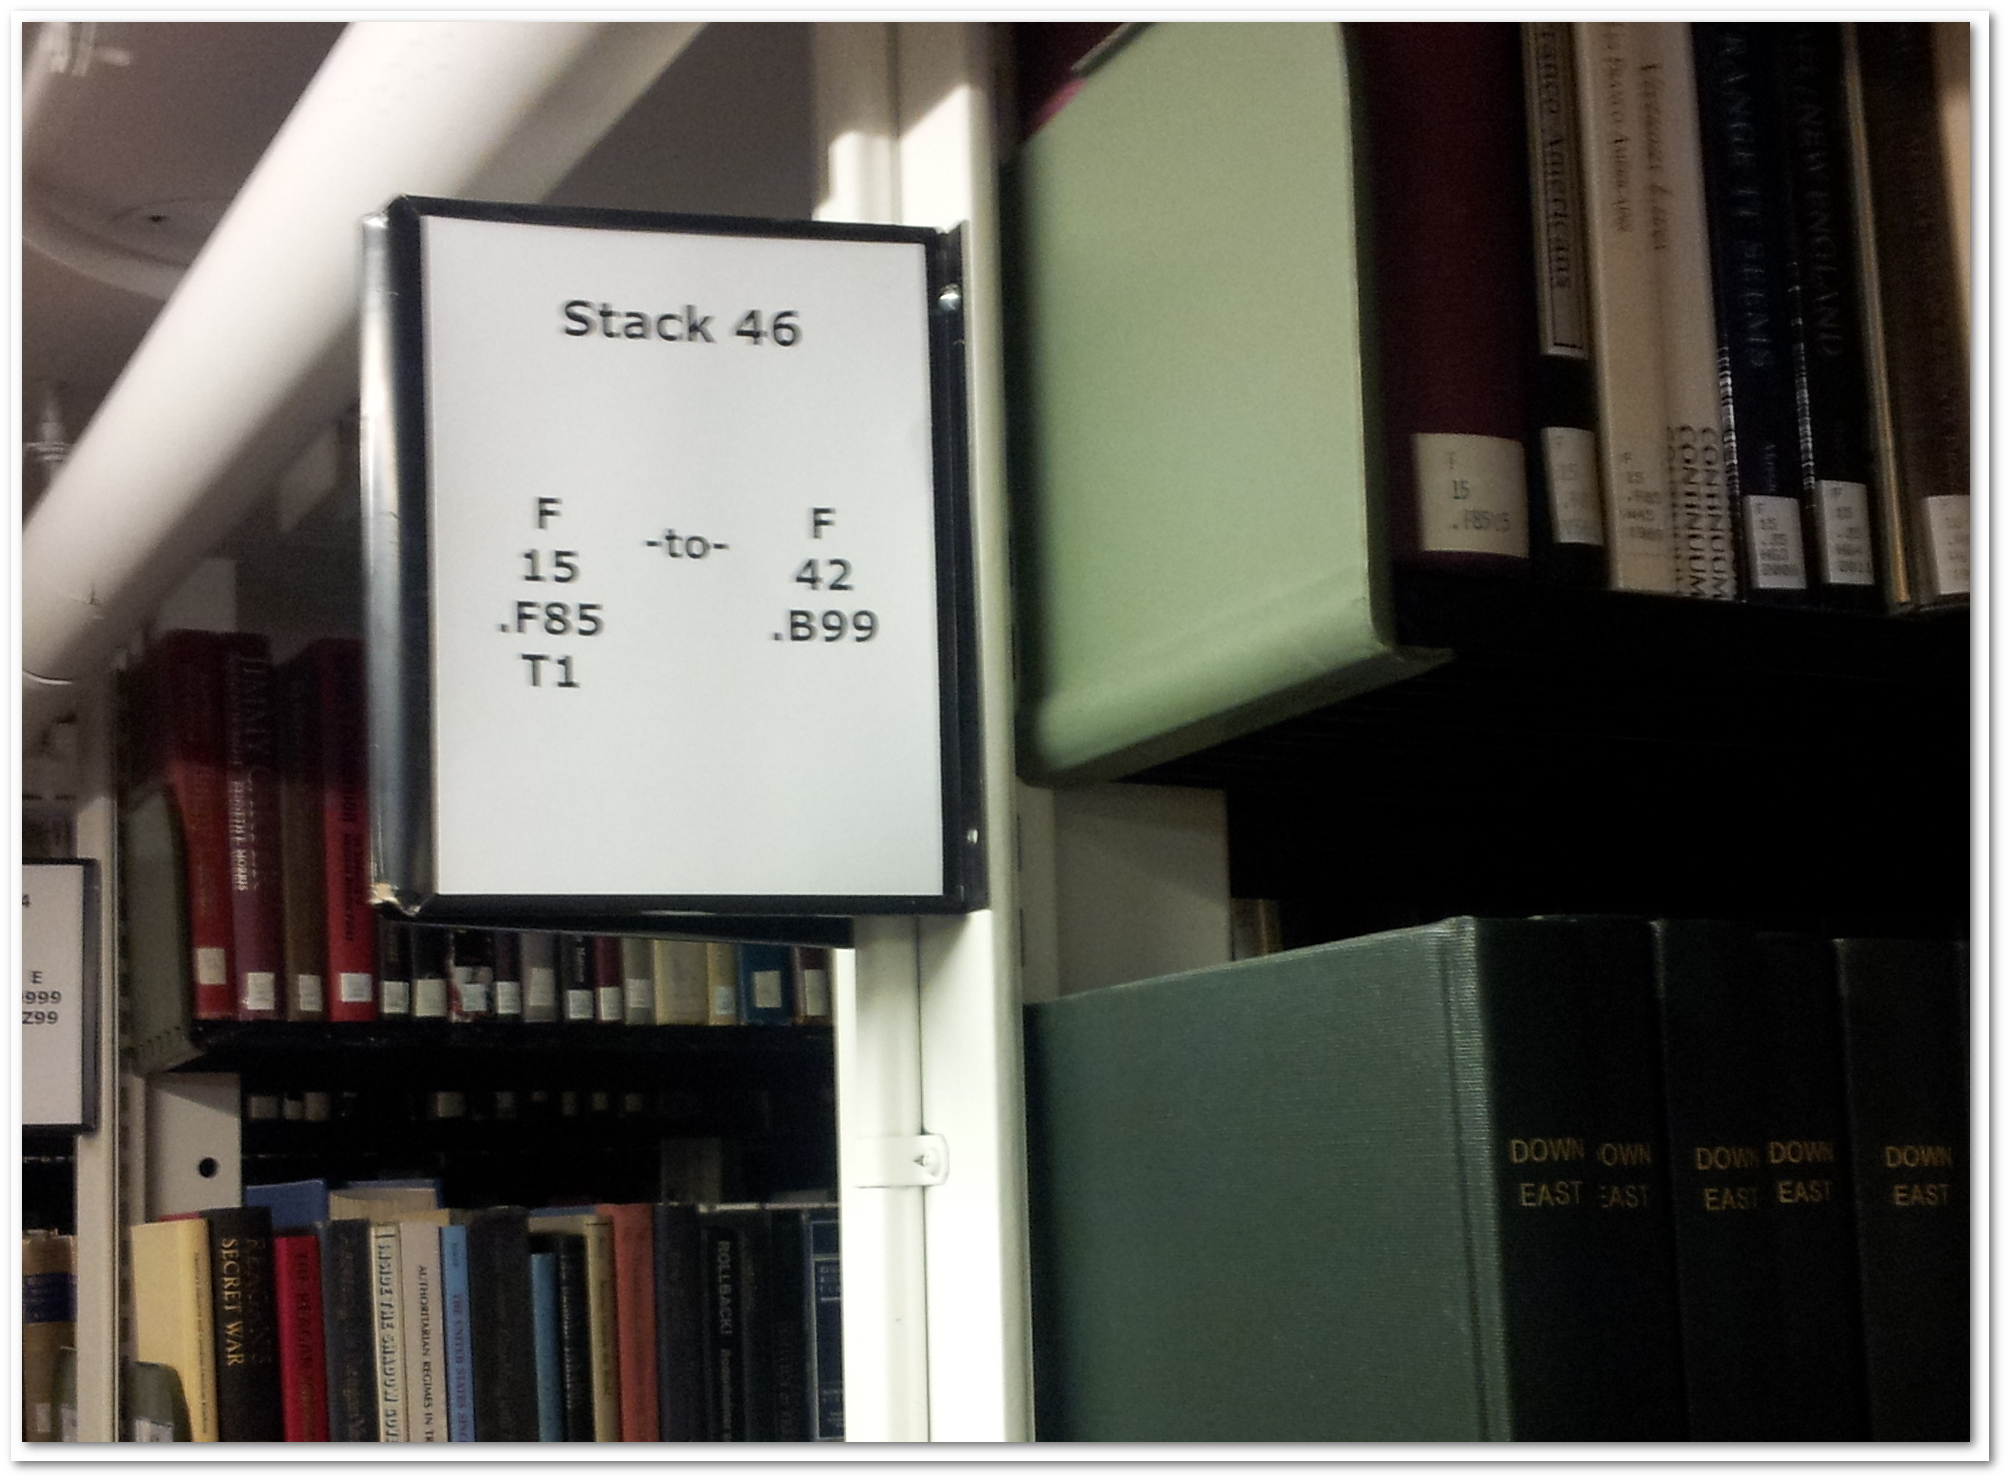
\includegraphics[scale=.15]{stacks}

{\small \{ \emph{Use these signs to determine if a book is in the row}. \}}

\end{center}



Since \textbf{F 24} is within this range, our example book is in that row. Once
in the proper row of shelves, proceed numerically until you find the 24s.
Finally, using the \textbf{Cutter line}, proceed alphabetically until you find
the Ts. Then proceed numerically until you find \textbf{.T39}, the address of our book.

As you can see, the call number should be read from left to right using
alphabetical and numerical orders. Thus, a book with a Subject line \textbf{F
}would be shelved \emph{before} a book with a Subject line \textbf{FA.}
Similarly, a Cutter line that reads \textbf{.T39} is shelved \emph{after}
\textbf{.T21}.

Maps of the library's floorplans are affixed to the walls on each floor. Free
paper maps of the library are available at the circulation desk of the library.
You may also consult the
\href{http://www.dartmouth.edu/~library/bakerberry/circ/stacksguides/}{maps and
floorplans} online with your computer or smartphone.

\begin{center}
\begin{tcolorbox}[colframe=oyster, coltitle=black, sharp corners, title=\ding{52} Note]
A new update to Dartmouth's catalog as of 2014
allows you to simply click the 
\includegraphics[scale=.6]{mapit} button next
to the item's listing. This will summon a map that shows you the exact location
of the book in the library stacks.
\end{tcolorbox}
\end{center}

\section{Sources our Library Doesn't Own}

A common problem in academic research is discovering that a book or article you
require for a project is checked out, missing, or not owned by the library.
There are a number of free services available to you when you encounter this
problem.

\subsection{Borrow Direct Consortium}

A number of the best libraries in the world have formed a consortium
designed to share resources and expand research opportunities for the  entire academic
community. As students of Dartmouth college, you may obtain  borrowing
privileges at any of the other participating libraries including Brown,
Columbia, Cornell, Harvard, Massachusetts Institute of Technology, University of
Chicago, University of Pennsylvania, Princeton, Yale and the Center for Research
Libraries. The combined resources total a staggering 50 million volumes.

To see if a book is available at another library, use a  service called
\href{http://www.dartmouth.edu/~library/res-share/borrowdirect/}{Borrow Direct}.
With this  service you may search every library in the consortium simultaneously
to see if the  book you require is available at another institution. If the book
is  owned by another school and is not checked out at the time, you may request
that the item be sent to our library. These requests usually arrive in 4 working
days or less.

\hypertarget{peer-review}{}

\subsection{DartDoc} If there is a book or article you would like to read that
is not available through Borrow Direct, you may request it from Dartmouth's
interlibrary loan program, known as DartDoc. To  request an item, visit the
\href{https://dartmouth.illiad.oclc.org/illiad/berry/logon.html}{DartDoc}
webpage, select the appropriate form (article, book, book chapter, etc.), and
send your request electronically to the office. Staff will
request your item from another library, who will ship the book to our library
through the mail. If you are requesting a book chapter or article, the donor
library will send you a .pdf free of charge to your DartDoc account.

\begin{center}
\begin{tcolorbox}[colframe=oyster, coltitle=black, sharp corners, title=\ding{52} Note]
If you are ordering a book, DartDoc is the
\emph{slowest} of all the  available options for requesting research materials.
Requests may take up to  two weeks to be fulfilled.
\end{tcolorbox}
\end{center}

\section{Research Guides}


If you are performing research on a topic and do not know where to begin,
Dartmouth's librarians have created an impressive collection of
\href{http://researchguides.dartmouth.edu}{Research Guides}  that can help you
find background information, periodical databases, and  academic journals
appropriate for your topic or discipline.


\section{Peer Review}

Peer review is a form of quality control in academic publishing. Before books
or articles are published, they experience a rigorous process of evaluation by
a number of experts who have advanced training in the field of study in
question. This scholarly review helps eliminate factual errors and other
problems before the works are published. Thus, peer-reviewed works are much more
trustworthy than other sources of information.

\subsection{Determining if a source is peer reviewed}

For novice researchers, distinguishing between \hyperlink{peer-review}{\color{Ahrenge}{peer-reviewed}} and other kinds of sources can be challenging. However, there are a number of things you can do to
ensure that you are using  peer-reviewed information. Many periodical databases,
such as  \href{http://dartmouth.idm.oclc.org/login?url=http://www.jstor.org/}{JSTOR}, only contain
peer-reviewed academic articles. Many other databases, such as
\href{http://dartmouth.idm.oclc.org/login?url=http://search.ebscohost.com/login.aspx?authtype=ip,uid&profile=ehost&defaultdb=a9h}{Academic
Search Complete}, have search limiters that can be selected to ensure  that the
search results only contain peer-reviewed sources. However, other  databases
lack clear indications about the nature of their sources. If you are  confused
about a source or database, ask your professor or one of the research
librarians for assistance.

If those are not practicable, use these test criteria: 

\begin{itemize} 

\item Scholarly, \hyperlink{peer-review}{\color{Ahrenge}{peer-reviewed}} articles almost always publish the university
affiliation of the professor/author/scientist.

\item Scholarly articles \emph{always} have a bibliography page.

\item Scholarly articles always contain citations and commonly have footnotes
or endnotes.

\item Generally speaking, if you can find the publication at the dentist's
office or on an airport magazine rack, then it isn't scholarly or
peer-reviewed. \emph{Time}, \emph{Newsweek}\textemdash even the \emph{New York
Times}\textemdash are not considered peer-reviewed sources. 

\item If the article contains advertisements, it is likely not scholarly. 

\end{itemize}

\section{The Oxford English Dictionary}

The \href{http://www.oed.com/}{OED} is, without question, the  greatest and most
complete dictionary ever created. As an historical dictionary, the OED systematically traces the  etymology of words in the English language.  \href{http://en.wikipedia.org/wiki/Etymology}{Etymology} is
"the study of the history of words, their origins, and how their form and
meaning have  changed over time." Thus, with the OED you can see when a word
entered or exited the English language and how its meaning evolved over time.

The OED is quite helpful when you are reading a novel, poem, or document that
was written in a time period distant from our own. Since words fall out of use
and the meanings of words change over time, it can often be difficult to
interpret the meaning of the texts we read from the past. The OED exists to
help us with this problem. You can think of it as a dictionary with a built-in
time machine.

\section{Helpful Research Suggestions}

\subsection{Not all sources are equal}

How do you know if you can trust your source? Here are some suggestions for
critically examining your sources:

\begin{itemize} \item \textbf{Examine the credentials of the author}. What is
the author's educational  background? Do they have an advanced degree in the
subject that they are  writing about? Are they affiliated with any major
institutions\textemdash such  as a university or government department? Does the
author have a respected  publication record that is frequently cited by other
experts in the field?

\item \textbf{Examine the date of publication}. When was the book or article
you are reading published? Since new discoveries and ideas are produced every
day, it is important to consult the most recent sources on your research
subject. Generally, the most current source should be preferred over older
sources.

\item \textbf{Determine if the source has been peer-reviewed}. Peer review is a
form of quality control in academic publishing. It ensures that the information
that is published has been properly evaluated and vetted by a number of other
professionals in the field. A peer-reviewed source should be preferred over any
other kind of information.

\item \textbf{Be wary of Internet sources}. If your source comes from the
Internet, you should take care to verify its trustworthiness. Most sites on the
Internet are not peer-reviewed sources of information. Misleading, politically
motivated, and even propagandistic content often masquerades as objective
information on blogs, websites, and discussion boards.  \end{itemize}

\subsection{Taking notes}

Now that you have some research materials in front of you, either at the
library or at home, it's time to make them useful to you. Before placing source
materials in your essay, \hyperlink{notes}{\color{Ahrenge}{take good notes}} by using \hyperlink{summary}{\color{Ahrenge}{summary}}, \hyperlink{paraphrase}{\color{Ahrenge}{paraphrase}}, and judicious \hyperlink{quotation}{\color{Ahrenge}{quotation}} to take ownership of the source materials. Ensure that
you cite appropriately and that your summaries and paraphrases use your own
original language. This intermediary step before writing the essay saves you
time and helps you avoid \hyperlink{plagiarism}{\color{Ahrenge}{plagiarism}}.

\begin{itemize}
\item If you'd like to keep organized notes on your computer, try the free and open-source
program called \href{http://rasm.ods.org/keepnote}{Keepnote}.
\end{itemize}

\subsection{Raid the Bibliography}

Occasionally, students find one or two sources on a topic and then despair of
finding any more. However, with just one excellent article or book, you can
easily generate additional research leads. When you find a book or article that
relates to your project, scour the bibliography to see what books and articles
the author used to produce his or her work. Make lists of the most promising
sources by writing down all the bibliographic information in a research
journal. Locate these sources in the library and then repeat the process. By
using this technique of routinely following up on sources cited in
bibliographies, you can generate a surprisingly large number of books and
articles on your topic in a relatively short time.

\subsection{Research Journal \& Bibliographic Software}

Keeping a research journal is an important habit to develop. Every student or
professor has had the unsettling realization that they have used a quotation in
their writing but have no recollection of where the quote came from. Many hours
can be consumed retracing steps. Frequently, source materials are never located
again. To avoid this problem, keep a research journal where you record the
bibliographic information of each source you read or browse. This way you can
quickly locate the information again.

Although a paper notebook works well as a research journal, there are some very
promising electronic alternatives. This bibliographic software can maintain a
record of your sources, help you take notes, and even produce perfectly
formatted bibliography pages for your essays.  \begin{itemize}\item For Mac
users, there is \href{http://www.sonnysoftware.com/}{Bookends}.  \item PC users
should consider \href{http://www.biblioscape.com}{Biblioscape}.  \item However,
the free and open-source option known as \href{http://zotero.org}{Zotero} is
perhaps the best option of all. \end{itemize}
